% !TeX spellcheck = en_GB
\documentclass[../summary.tex]{subfiles}

\begin{document}
	
	\section{Economics for sustainability}
	
	\subsection{Study guide}
	
	This chapter will be on the connection between economy and environment and the shortcomings and opportunities of economics for sustainable development. The study guide for this chapter of the MOOC was a complete mess and basically covered the whole transcript. That is why, even though this part of the summary is still based on the study guide, there won't be a structured overview of it.
	\\\\
	Typical questions for this chapter are:
	\begin{itemize}
		\item Definitions, terminology: be able to explain the definition, give examples
		\item Graphs: be able to explain and interpret the graphs
		\item Principles: be able to explain, give examples
	\end{itemize}
	
	\subsection{Gross Domestic Product}
	\label{sec:10-gdp}
	
	The \textbf{Gross Domestic Product} or \textbf{GDP} is a measure of total production that is used to reflect the economic health of a country or region and has strongly increased since the end of the 19th century. Figure \ref{fig:GDP} shows this exponential growth.
		
	\begin{figure}[htbp]
		\centering
		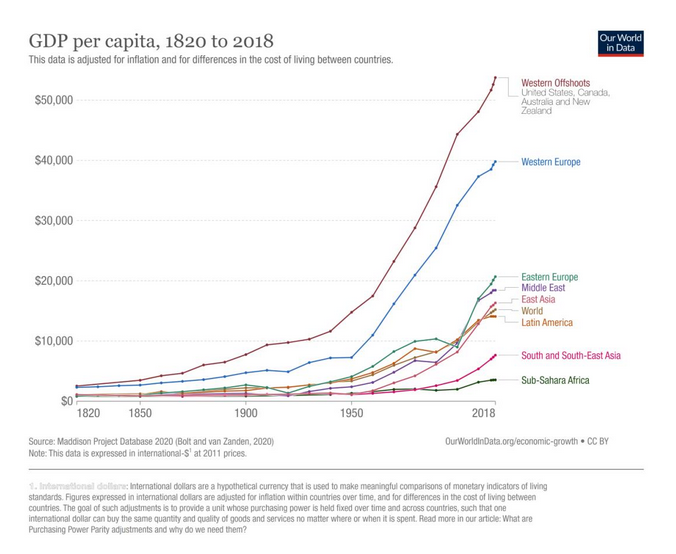
\includegraphics[width=1\linewidth]{images/10-GDP-increase.png}
		\caption{Increase in GDP since 19th century}
		\label{fig:GDP}
	\end{figure}
	
	\newpage
	This increase in GDP went together with a lot of other positive phenomena, such as an increase in life expectancy, an increase in literacy, a decrease in hunger, and so on. However, at the same time, we also saw a rise in environmental pressures, such as greenhouse gas emissions, global warming, plastic pollution, declining biodiversity, and many more. 
	\\\\
	\textbf{Economic growth} is the annual percentage change of real GDP. Real GDP means it's GDP measured in monetary terms, but it's corrected for inflation and price changes.
	\\\\
	There are multiple ways to define GDP. The first approach is the so-called \textbf{added value approach}. We define GDP as the value of all final goods and services that are produced in a given country in a given period of time. A second way to define GDP is to look at incomes. All that value added in the GDP is giving rise to incomes, incomes to the persons who own the factors of production. Factors of production are labour, capital and land. So in the second approach to GDP, the \textbf{income approach}, GDP can be defined as the sum of all the incomes that are earned by the owners of factors of production in a given year, in a given country. 
	\\\\
	We should look at GDP as \textbf{a measure of production and of economic activity}. It was not intended to be a measure of prosperity or well-being or happiness. So \textbf{a lot of things are not picked up by the concept of GDP}. A first example of something that is missing in the GDP is a good idea about the distribution or the inequality. A second thing which is missing from the GDP is unpaid work. A third element that is not included in the GDP are changes in the quality of the environment.
	\\\\	
	Figure \ref{fig:emissions-and-GDP-per-capita} shows the emissions and GDP per capita for the different countries. Looking at the graph, we can see there seems to be an increasing relationship between GDP per capita and emissions per capita. Richer countries, with a higher GDP per capita, have higher emissions per capita. We can also see that the big countries, like China and India, are on an intermediate level of emissions. If we study the evolution of the emissions versus the GDP per capita during the 20th and 21st century, like depicted on Figure \ref{fig:emissions-and-GDP-per-capita-long-term}, we notice two different trends. Countries like China and India started at a low level of both emissions and GDP per capita, but they gradually increased over time and are still increasing. On the other hand, we have countries like Belgium and the United States that started increasing at an intermediate level of emissions per capita, but then reached a peak and started decreasing. This pattern is observed for many developed economies and the idea behind it is the so-called Kuznets curve
	
	\begin{figure}[htbp]
		\centering
		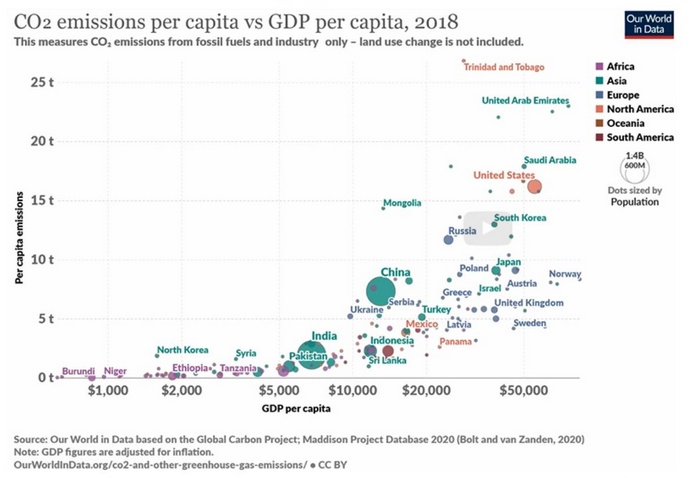
\includegraphics[width=0.9\linewidth]{images/10-emissions-and-GDP-per-capita.png}
		\caption{$CO_{2}$ emissions per capita versus GDP per capita, 2018}
		\label{fig:emissions-and-GDP-per-capita}
	\end{figure}
	
	\begin{figure}[htbp]
		\centering
		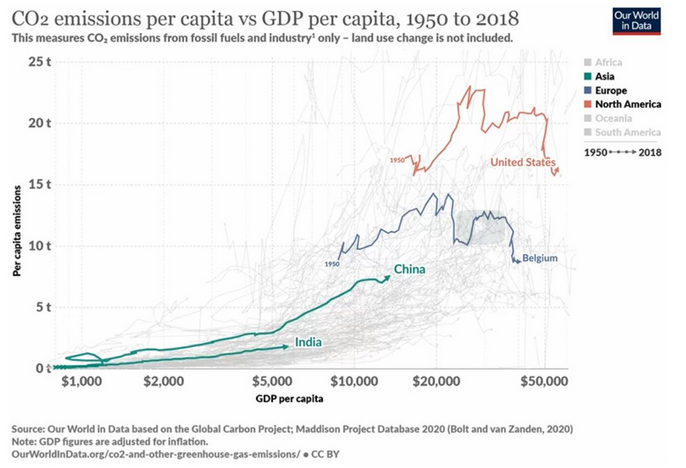
\includegraphics[width=0.9\linewidth]{images/10-emissions-and-GDP-per-capita-long-term.png}
		\caption{$CO_{2}$ emissions per capita versus GDP per capita, 1950 to 2018}
		\label{fig:emissions-and-GDP-per-capita-long-term}
	\end{figure}

	\subsection{The Kuznets curve}
	
	 Like we mentioned in section \ref{sec:10-gdp}, the \textbf{Kuznets curve} is used to describe the pattern we see in the evolution of emissions and GDP per capita for countries with developed economies. The Kuznets curve is typically an inverted U-shape of form (Figure \ref{fig:emissions-and-GDP-per-capita-long-term}), meaning that initially countries have very low emissions per capita and GDP per capita. But then they start to economically develop, and they start to industrialize. During that industrialization phase, we see rapidly increasing emissions in per capita terms, but also rapidly increasing GDP per capita. At a certain time, there typically comes a moment when economies start to shift away from this heavy industry towards other activities, like, for instance, services. This means that the emission intensity of that economy is gradually decreasing and the growth of their emissions is also decreasing. This can also be influenced by governments that are stepping in and are developing environmental policies to combat pollution. This evolution of first \textbf{increasing, peaking and then decreasing emissions}, that is what we call the Kuznets curve. 
	 \\\\
	 However, it is important to note that this curve is a correlation, and not a causal relationship. Hence, we can't just simply say that the low-income countries just need to focus on growth in order to solve the solution problems.
	 \newpage
	\subsection{Production versus consumption based emissions}
	
	We can make a distinction between production and consumption based emissions. Up until this moment, we have been looking at emissions in the production perspective. \textbf{Production perspective emissions} are a measure of emissions within a given territory of a particular country. However, this is not the full story because we are not only consuming goods that are produced in our country but are also consuming goods imported from other economies. The emissions of these imported goods are not considered in the production perspective we have used so far. If we want to get a fairer approach of our emissions, we should also consider this. This is done by the \textbf{consumption perspective}.
	\\\\
	If we look at our country, we can see that the consumption based emissions are very high. The production based emissions of Belgium are intermediate. For other (production-based) countries like China, we see the opposite. If we calculate the absolute level of emissions, we get an overview of the actual emissions we are causing. We can call this our \textbf{carbon footprint}.
	
	\subsection{Drivers of environmental impact}
	
	If we want to take a look at the drivers for $CO_{2}$ emissions, we first start with the \textbf{IPAT relationship}. This relationship says that environmental impact (I) is the product of 3 drivers: population (P), affluence or GDP per capita (A) and technology (T). The product of these 3 drivers gives rise to the environmental impacts. A special case of this IPAT relationship is the \textbf{Kaya decomposition} of greenhouse gas emission evolution. This decomposition makes a more sophisticated distinction between two technological drivers. Hence, it states the $CO_{2}$ emissions can be written as a product of 4 factors.
	\\\\
	Like previously mentioned, the first driver is \textbf{population}. The more people there are, the more goods and services are produced and the more $CO_{2}$ will be produced. 
	\\\\
	The second driver is GDP per capita. This is a measure of \textbf{affluence}. When people get richer, they typically demand more goods and services which will also result in a rise of emissions.
	\\\\
	In terms of \textbf{technology}, the Kaya decomposition makes a distinction between energy intensity and $CO_{2}$ intensity of energy production. The \textbf{energy intensity} measures how much energy we need to produce one unit (for example $\$1$) of GDP. Unlike the previous factors, we expect the energy intensity to go down over time because our economy becomes more of a service economy instead of an industrial economy and because of technological progress. \\\\
	The \textbf{$CO_{2}$ intensity of energy production} measures how much $CO_{2}$ is released by producing one unit of energy. Since we are currently decarbonizing our energy production by investing in solar panels and wind energy, we also expect this to go down over time.
	\\\\
	Figure \ref{fig:Kaya-decomposition-world} shows the actual global reality of these different factors and their evolution. We can see that the emissions and the GDP grow at the same percentage rate, so there is no decoupling between them. If we look at this evolution for Belgium, we can see that this is not the case. For Belgium, the curves are separating and there is \textbf{absolute decoupling}: whereas on the one hand GDP per capita is still growing, we see that emissions are going down in absolute amount. A \textbf{relative decoupling} would mean that emissions are growing but at a slower pace than the GDP per capita. When we look at the different Kaya factors, we see the same trend as described before for the global overview, with one difference: our population is growing a lot slower than the global population. This results in slightly decreasing $CO_{2}$ emissions since 1990. We can see this in Figure \ref{fig:kaya-decomposition-belgium}.
	
	\begin{figure}[htbp]
		\centering
		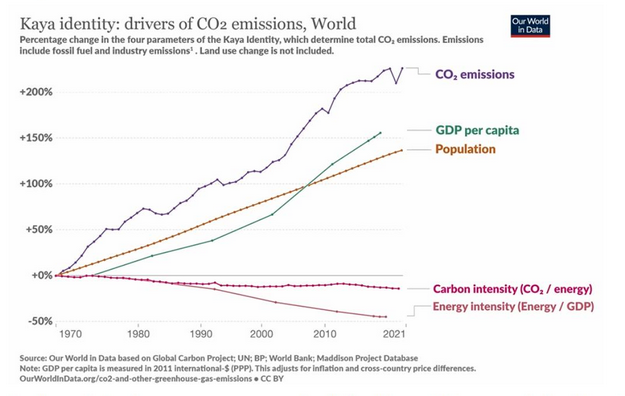
\includegraphics[width=1\linewidth]{images/10-kaya-decomposition-worldwide.png}
		\caption{Kaya decomposition (worldwide)}
		\label{fig:Kaya-decomposition-world}
	\end{figure}
	
	\begin{figure}[htbp]
		\centering
		\includegraphics[width=1\linewidth]{images/10-Kaya-decomposition-belgium.png}
		\caption{Kaya decomposition (Belgium)}
		\label{fig:kaya-decomposition-belgium}
	\end{figure}
	\newpage
	\subsection{Frameworks of sustainable development}
	
	Brundtland defines \textbf{sustainable development} as a development that meets the needs of the present generation without compromising the ability of future generations to meet their own needs. In order to make the concept of sustainable development more operational, we will make a distinction between so-called weak and strong sustainability. But before we do this, we will first introduce the \textbf{different types of capital in economics}.
	\\\\
	 A first concept of capital is \textbf{physical capital}. This type of capital is the physical infrastructure (roads, bridges, ports, canals, but also data networks and so on).
	 \\\\
	 The second type of capital in economics stems from labor, specifically the number of people and their skills. We call this \textbf{human capital}.
	 \\\\
	 Furthermore, there is also the \textbf{natural capital}. This type of capital is generally linked with our renewable and non-renewable sources and level of pollution.
	 \\\\
	 Lastly, we also consider the institutional or \textbf{social capital}. This is about the institutions, police, legal system, judges and so on in a society.
	 \\\\
	 Now, we are able to define \textbf{weak sustainability}. A development path is called weakly sustainable if the total sum of natural, human, physical and social capital is not decreasing over time. If you use a weak concept of sustainability, then you basically allow for substitution between different compartments of capital. For example, it's possible that your natural capital is decreasing, but over-compensated by an increase in another capital stock.
	 \\\\
	 In \textbf{strong sustainability} we require that each of the four capital stocks on their own are non-decreasing over time. So in that case it's not possible anymore that a decrease in one would be compensated by an increase in another capital stock. All of them have to be non-decreasing over time and there can be no erosion.
	 \\\\
	 A first practical example of sustainable development is the \textbf{Adjusted Net Savings} by the World Bank. This concept tracks the evolution of different capital stocks over time on a country level. They make a distinction between the changes in physical, natural and human capital and then make the sum of these changes. If that total sum is positive, we can say that the adjusted net savings are positive and that this country is on a sustainable development track. Clearly, this is an example of a weak sustainability concept because we add the changes in the different capital stocks together. So a decrease in one can be compensated by an increase in another one.
	 \\\\
	 Another example is the \textbf{donut economy concept} of Kate Raworth. This concept is visualised on Figure \ref{fig:donut-economy} and will be explained more detailed in Chapter 11. The outer ring is the environmental sustainability. The economy should not grow out of this environmental safe operating zone. The inner circle refers to the social aspect of the society and the justice elements. Society should not infringe upon the rights and the social and the justice needs of all the members of our society. Hence, this band basically defines the safe and the just space for society to operate in. Looking at the outer ring, we can clearly here see an example of strong sustainability, because this concept is about the safe operating zone in different compartments - biodiversity, climate change and so on - that the society should respect. So here we have an example of a concept that does not allow for trespassing the safe operating zone, and also it does not allow for compensation between the different types of capital in the society. 
	 
	 \subsection{Externalities}
	 
	  In economics, we speak of an \textbf{externality}, if a production or consumption activity of an economic agent is affecting the consumption or production possibilities of another economic agent without full compensation being paid through the market mechanism. 
	  \\\\
	  An \textbf{example of influence of other production} is paper production that is affecting negatively the production possibilities of another production facility, the fish farm by dumping toxic chemicals and wastewater in the river, which then flows into the sea. Now imagine that downstream people are living along the river, normally enjoying a very nice scenic view on the water. But because of the water pollution, the water might be stinking and that is obviously negatively affecting the consumption possibilities of the homeowners. They can't enjoy a nice barbeque anymore in their garden, for example. So that is an \textbf{example of a production activity negatively affecting consumption possibilities}. This example also allows us to introduce the \textbf{compensation condition}.  Imagine that the homeowner bought his house at a discount because he knew that it would be affected by this negative externalities by the bad smell of the polluted water. So he paid less than what he would normally do for such a nice house. That price discount is to some extent compensating for the externality. So if the price discount would be fully compensating the externality, then the discount is basically cancelling the externality, and we cannot speak any more of an externality. It's only when the discount is less than the value of externality, then there will still be some remaining externality. That is why this last condition of compensation is important in the definition of an externality.
	  \\\\
	  Next, we can take a look at \textbf{how externalities influence the principle of a normal market of supply and demand} and how they can lead to market failure. \textbf{Market failure} means that the outcome of the market interaction is leading to an allocation that is not optimal from the point of society.
	  \\\\
	  In a normal market of supply and demand, we will get a downward sloping curve for the demand of our product if we plot the quantity on the horizontal axis and the price on the vertical axis, like on Figure \ref{fig:influence-externalities}. The higher the price, the lower the bought quantity will be and vice versa. This is the demand side. The supply side is an upward sloping, marginal private production cost curve. This is  reflection of the cost produce the product. Extra production requires extra input, hence an upward sloping curve. Without any government intervention or regulation, market equilibrium will occur at the intersection of demand and supply (point $E_{0}$ on Figure \ref{fig:demand-supply}). If externalities are present, the supply curve will be positioned higher then before. This result in a quantity that is to high ($Q_{0} > Q^{*}$) and a price that is to low ($P_{0} < P^{*}$) for what is optimal for society. This is shown by Figure \ref{fig:demand-supply-externality}. We can say that the free market prices are not properly reflecting the marginal external climate change costs of production and that's why we end up with a market failure.
	  
	  \begin{figure}[htbp]
	  	\centering
	  	\begin{subfigure}{.5\textwidth}
	  		\centering
	  		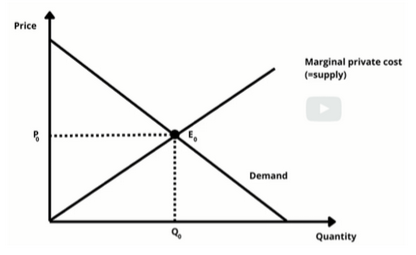
\includegraphics[width=1\linewidth]{images/10-demand-supply.png}
	  		\caption{Without externalities}
		  	\label{fig:demand-supply}
	  	\end{subfigure}%
	  	\begin{subfigure}{.5\textwidth}
	  		\centering
	  		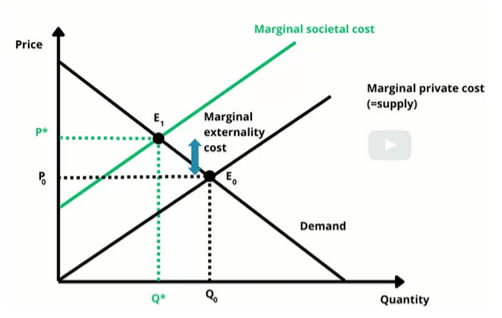
\includegraphics[width=1\linewidth]{images/10-demand-supply-externalities.png}
	  		\caption{With externalities}
	  		\label{fig:demand-supply-externality}
	  	\end{subfigure}
	  	\caption{Influence of externalities supply/demand market}
	  	\label{fig:influence-externalities}
	\end{figure}
	 
	 \subsection{Public goods}
	 
	  A \textbf{public good} is a good that is characterized by two crucial characteristics. The first is non-rivalry and secondly non-excludability. Public goods are \textbf{non-rival}, meaning that the consumption of that good by an individual does not reduce the amount available for others to consume of that good. A second characteristic of a public good is that it is \textbf{non-excludable}. It is not possible to prevent people from consuming the public good. 
	  \\\\
	  We can consider \textbf{lower emissions as a public good}. If countries reduce their emissions, that will lead to lower concentrations of greenhouse gases in the atmosphere and in the end, in the future, that will lead to less climate change. So that's clearly a benefit. This lower degree of climate change is a public good in the sense that it is non-rival. If one country like Belgium or Europe enjoys a better climate that does not prevent China or the US or Africa from enjoying a better climate. It’s also non-excludable. Imagine that the US would not want to contribute emission reduction efforts to lower the greenhouse gas emissions, then still they can enjoy the benefits of a better climate.
	  \\\\
	  This will lead to \textbf{free riding behaviour}. If an actor, a country, knows that it cannot be prevented from enjoying the benefits of a public good once it is provided, that makes it very tempting to refuse to contribute. 
	  \\\\
	  We can illustrate this incentive to free riding with an \textbf{example of two countries} that are thinking about joining and contributing to an international agreement of emission reduction: the USA and China. They both have the option to contribute or to free ride. This gives us the payoff matrix we can see in Figure \ref{fig:payoff-matrix}. We can now discuss the 4 different possibilities from the point of view of the US. The first situation is the one where the USA free rides and China contributes. For the USA, this is the most desirable outcome. If the USA also contributes, we get situation 2. This is also desirable, because it as a positive effect on the emission reduction, but less then the first situation because now the USA also needs to contribute. If both countries are free riding (situation 3), there will be a bad outcome for the climate, but not for the countries themselves. The worst situation for the USA would be situation 4, where the USA contributes and China free rides. This payoff matrix can be used to determine what is the optimal strategy of the US to play in the negotiation game, based on the behaviour of China.
	  
	  \begin{figure}[htbp]
	  	\centering
	  	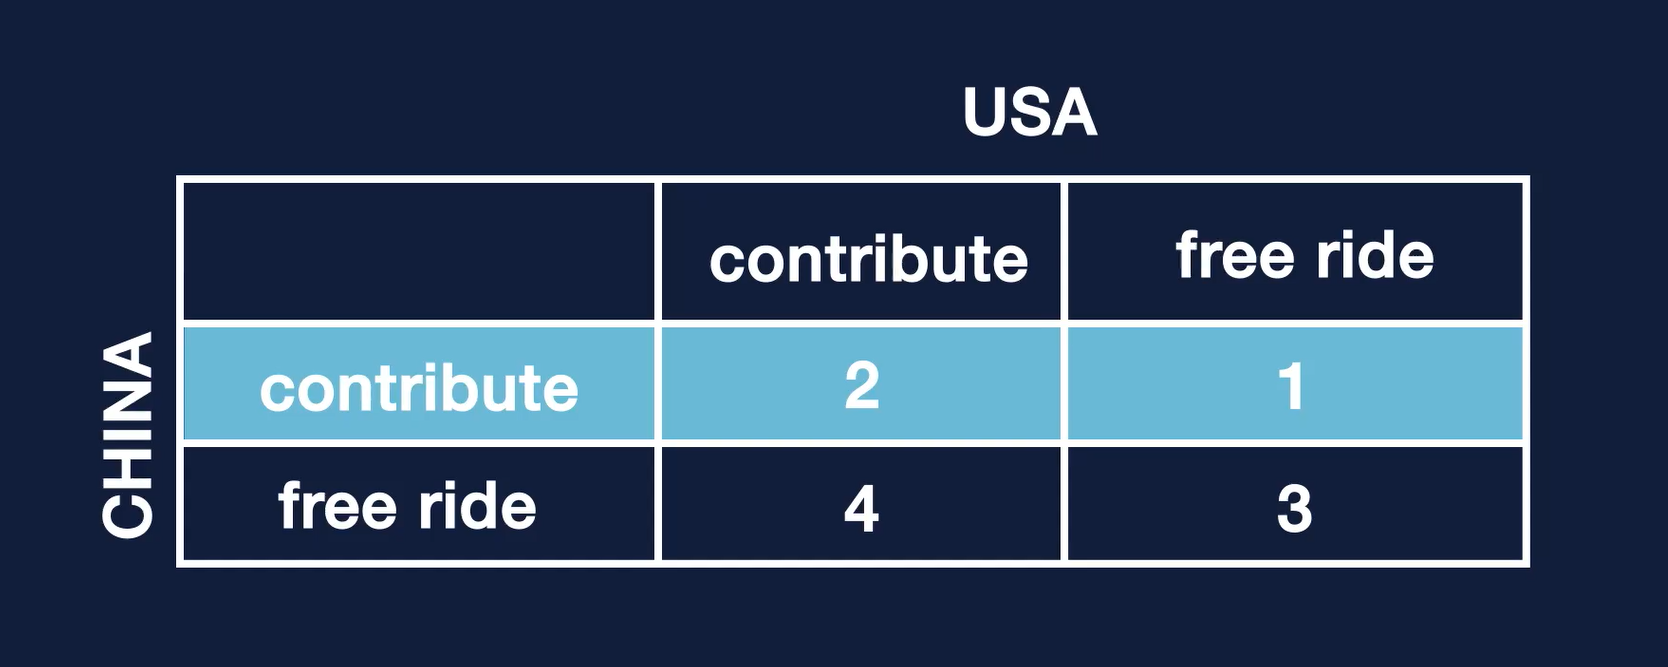
\includegraphics[width=1\linewidth]{images/10-payoff-matrix.png}
	  	\caption{The payoff matrix between the USA and China}
	  	\label{fig:payoff-matrix}
	  \end{figure}
	  
	  Given this urge to free ride, there is a strong reason to call for government intervention to prevent market failure. This works fine at the \textbf{national level}. We have national governments that produce a lot of public goods (think about defense and education, legal system, public infrastructure and so on). These public goods are financed it with compulsory taxation, paid by every citizen. However, at \textbf{international level}, we don't have those strong governments. So all cooperation on the provision of global public goods has to come from voluntary contributions and voluntary agreements like the Paris Protocol. That is why it will be very challenging to overcome this free riding incentive on an international level.
	  
	  \subsection{Elinor Ostorm}
	  
	  An important name in this field of research is Elinor Ostrom. Her research focused primarily on the management of local commons (or public goods). Her main contribution is that she shows that communities often succeed in managing commons in a sustainable way without government intervention.
	  \\
	  Instead of the classic dichotomy between the market and the government, Ostrom showed that there is often a third option in which the users of a natural resource themselves set up sophisticated decision-making and enforcement systems to resolve their conflicts of interest. In this sense, her work complements the classical view that non-excludability inevitably leads to overexploitation of commons in the absence of government action. This classical view is called the tradegy of commons. 
	  \\\\
	  The numerous examples of successful and sustainable management of commons that Ostrom cites are usually about relatively small local communities such as a fishing village or a small farming community managing a common pasture or forest. In such communities, mechanisms, formal or informal or otherwise, often exist to enforce restrictions on the use of the natural resource. Those who do not comply with catch limits may risk being expelled from the community. And those who do not belong to the community may be denied access to the resource, sometimes by force. But for global commons with numerous potential users such as, for example, the atmosphere to emit greenhouse gases or tuna stocks in international waters, high coordination and transaction costs often prevent the emergence of effective management mechanisms. In such cases, the tragedy of the commons still looms.
	  
	  \subsection{Environmental policy}
	  
	  We can conclude that externalities and public goods can cause markets to fail. That's why there is a need for public intervention to restore optimality. There are different ways governments can intervene in markets: \textbf{regulation, prohibition, subsidies, taxes} (and combinations of these).
	  
	  \subsection{Cost efficiency}
	    
	  In order to explain the concept of cost efficiency, we will first introduce the concept of a marginal emission reduction cost curve, or a so-called MAC curve. Typically there are many, many different ways to reduce emissions and they typically differ in terms of the costs that they entail, but they also differ in the emission reduction potential that they can bring. A \textbf{marginal abatement cost curve (MAC)} is a concept or a device that helps you to trade off these different projects against each other.
	  \\\\
	  We can compare two different ways to reduce emissions for the example case of 2 companies. The first way is to impose \textbf{identical reductions} to the 2 companies. Since the cost of the different reduction processes is not the same, the total cost for both companies will not necessarily be the same. In this example we can see on Figure \ref{fig:reduction-identical} that the Green company has a cost of 80, while the Blue company only has a cost of 42. A better way would be to base the reduction on \textbf{marginal cost}. Using this way, the Blue company will need to do more effort than the Green company, but the cost will be the same for both companies. This way is shown on Figure \ref{fig:reduction-marginal-cost}.
	  
	  \begin{figure}[htbp]
	  	\centering
	  	\begin{subfigure}{.5\textwidth}
	  		\centering
	  		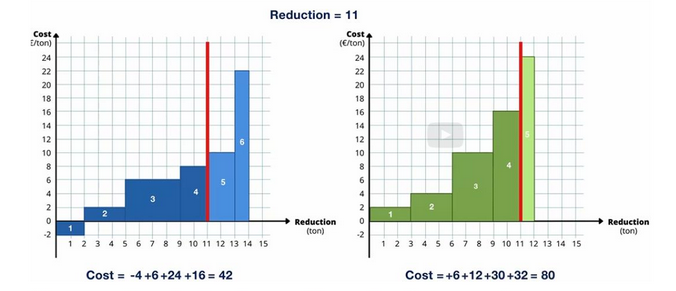
\includegraphics[width=1\linewidth]{images/10-identical-reduction-for-companies.png}
	  		\caption{Identical reductions}
	  		\label{fig:reduction-identical}
	  	\end{subfigure}%
	  	\begin{subfigure}{.5\textwidth}
	  		\centering
	  		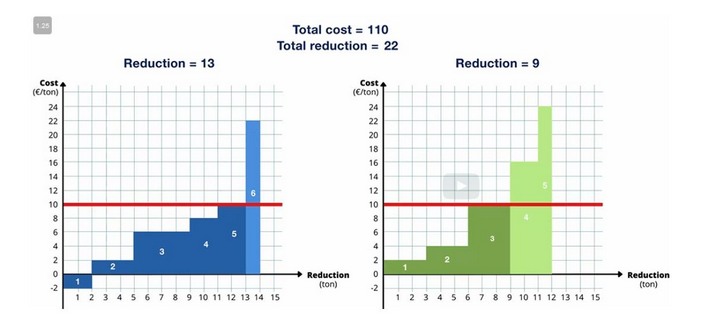
\includegraphics[width=1\linewidth]{images/10-reduction-based-on-marginal-cost.png}
	  		\caption{According to marginal cost}
	  		\label{fig:reduction-marginal-cost}
	  	\end{subfigure}
	  	\caption{Total cost when imposing two different ways for reduction}
	  	\label{fig:reduction}
	  \end{figure}
	  \newpage
	  \subsection{Price based instruments versus legal standards}
	  
	   A big difference between price based instruments and standards is that \textbf{price based instruments} are more \textbf{cost efficient}. This means that the total cost to society to reduce emissions to a given level is as low as possible. Legal standards are in most cases not cost efficient because it's very difficult for a regulator to know of each company its individual technology options. Usually the regulator will use a sector average to define the emission standards. And so that leaves a lot of options for cost savings aside.
	   \\\\
	   A second criterium to look at when it's about the choice of policy instruments is \textbf{dynamic efficiency}. If you are confronted as a company with a emission tax on your remaining emissions, that means that every year you are reminded of the cost of this remaining emissions. So every year you get the signal that there are perhaps other options to reduce your emissions even further, because perhaps new technologies have come on the market to reduce your emissions or existing technologies have become cheaper. So you are continuously reminded that there are perhaps ways to improve your environmental performance, because you are all the way you are every time you are taxed on the remaining emissions. That is very different with the emission standards.
	   \\\\
	   Hence, we can conclude there is a difference between price based instruments and legally enforced emission standards in the sense of dynamic efficiency and static cost efficiency. In both cases, we see that price based instruments perform better than legal standards.
	  
	  \subsection{Green tax reform}
	  
	  When a government introduces carbon tax, we will notice that the tax triggers users to implement reduction projects, but it also can be used with a sustainability impact. 
	  \\\\
	  The government could use some of the carbon tax revenue in order to give subsidies to households to invest in solar PV on their rooftop or to help companies to build wind turbines or to invest in energy efficiency of their installations. 
	  \\\\
	  A second possible use of the revenues of a carbon tax is to invest in social policy. And that can be very important because we know that introducing a carbon tax is typically regressive. With regressive we mean that it can make the income distribution even more unequal. The reason for that is that energy related expenditure related to fossil fuels are, in percentage terms, more important for poor households in their budget than the share of that in rich household budgets. So if we then introduce a carbon tax that will weigh more heavily on the shoulders of the poorer households than on the richer households. 
	  \\\\
	  A third possible use of the tax revenue of a carbon tax is to use it for labor market policies. In a lot of European countries we are seeing very high rates of labor taxes. And this is giving a disincentive for people to go out working and also giving a disincentive to employers to create new jobs. So this is holding back a lot of economic activity.
	  \\\\
	  The \textbf{double dividend} is the idea that by combining a carbon tax with lower labor taxes, we can achieve a win win situation. A first dividend is lower environmental pressure, lower emissions, a better environment because of the taxation of carbon. The second benefit or dividend has to do with the labor market. Because we invest the revenue in lower labor taxes, we will see more jobs. So better environment combined with more jobs.
	  \\\\
	  The general idea for green tax reform is tax bads (carbon dioxide or other environmental pollution problems) and not goods (for instance, labor).
	  \newpage
	  \subsection{Taxes versus subsidies}
	  
	  Taxes and subsidies, disencouraging the bad and encouraging the good alternative seem equally effective, but they are not. There are two rebound effects we can notice. The \textbf{first rebound effect} is that subsidies are partly effective, but miss the underlying consumption activity. Think about giving subsidies for electric cars. This will give incentive to green behaviour, but doesn't give disincentive for private mobility, which is the underlying consumption activity. The \textbf{second rebound effect} is that subsidies are an extra budget that may be used for carbon intensive activities. Think about giving big subsidies to households, which can give them incentive to use the additional budget to go on a trip to Barcelona for example.
	  \\\\
	  This is not the only problem with subsidies. Subsidies should trigger investments that would not be taken without subsidies. In reality, this is not always guaranteed. This is the problem of \textbf{additionality}. An other downside to subsidies is \textbf{the Matthew effect}. Subsidies should impact the poorer part of society, but the often have higher impact on the richer part. Furthermore, subsidies are expensive for governments, and often lead to higher taxes, especially on labor.
	  \\\\
	  Before we conclude if taxes are better than subsidies or not, we will take a look at existing environmentally harmful subsidies in our tax scheme. A first example of bad subsidies or bad tax exemptions are salary cars. Employees are given cars almost free (and with a tax exemption) from their employer, which is nice, but leads to a lot of additional traffic, traffic jams, accidents and also emissions. Another example are the subsidies for non-sustainable agricultural activities. Getting rid of these subsidies would be a start in the right direction.
	  \\\\
	  Another step is a carbon tax improvement. Right now, different energy consumption are taxed in different ways because they are submitted to different tax systems. Because of this, 30\% of energy use is not taxed, while others are taxed at high rates.
	  
	  \subsection{Link with other challenges}
	  Since economics and sustainability are such broad topics, we can find a lot of links with the other domains we studied earlier. A first link we can find is one with \textbf{climate and biodiversity}. The market uses to much fossil fuels because its negative externalities are not taken into account and it does not provide enough effort for biodiversity because its positive externality is not taken into account. Furthermore, the principle of freeriding makes greenhouse gas reduction very difficult. We can also find a link with \textbf{demography}. A better economy will lead to a higher GDP, which will lead to a higher population and higher emission/capita, which will then result in higher CO2 emissions. It is difficult to avoid this chain. The third link we can find is the link with \textbf{buildings} and \textbf{mobility}. The market brings too much car traffic because negative externalities are not taken into account. Smart road pricing might be a solution for this problem. Secondly, subsidies for salary cars are an example of bad subsidy. Another link we can find is the one with \textbf{raw materials} and \textbf{circular economy}. The market leads to lots of material extraction because negative externalities are not taken into account. There also is a deposit refund system for one way packaging. The last link we will cover is the link with \textbf{energy}. PV, battery and electric car subsidies suffer from the Matthew effect. Also, the energy of heating households is not taxed in a good way. The taxation of all energy carriers
	  should be aligned with full social cost.
	
\end{document}